%╔════════════════════════════╗
%║	  Szablon dostosował	  ║
%║	mgr inż. Dawid Kotlarski  ║
%║		  16.10.2021		  ║
%╚════════════════════════════╝
\documentclass[12pt,twoside,a4paper,openany]{article}

    % ------------------------------------------------------------------------
% PAKIETY
% ------------------------------------------------------------------------

%różne pakiety matematyczne, warto przejrzeć dokumentację, muszą być powyżej ustawień językowych.
\usepackage{mathrsfs}   %Różne symbole matematyczne opisane w katalogu ~\doc\latex\comprehensive. Zamienia \mathcal{L} ze zwykłego L na L-transformatę.
\usepackage{eucal}      %Różne symbole matematyczne.
\usepackage{amssymb}    %Różne symbole matematyczne.
\usepackage{amsmath}    %Dodatkowe funkcje matematyczne, np. polecenie \dfac{}{} skladajace ulamek w trybie wystawionym (porównaj $\dfrac{1}{2}$, a $\frac{1}{2}$).

%język polski i klawiatura
\usepackage[polish]{babel}
%\usepackage{qtimes} % czcionka Times new Roman
\usepackage[OT4]{polski}
%\usepackage[cp1250]{inputenc}                       %Strona kodowa polskich znaków.

%obsługa pdf'a
\usepackage[pdftex,usenames,dvipsnames]{color}      %Obsługa kolorów. Opcje usenames i dvipsnames wprowadzają dodatkowe nazwy kolorow.
\usepackage[pdftex,pagebackref=false,draft=false,pdfpagelabels=false,colorlinks=true,urlcolor=blue,linkcolor=black,citecolor=green,pdfstartview=FitH,pdfstartpage=1,pdfpagemode=UseOutlines,bookmarks=true,bookmarksopen=true,bookmarksopenlevel=2,bookmarksnumbered=true,pdfauthor={Dawid Kotlarski},pdftitle={Praca Inznierska},pdfsubject={},pdfkeywords={transient recovery voltage trv},unicode=true]{hyperref}   %Opcja pagebackref=true dotyczy bibliografii: pokazuje w spisie literatury numery stron, na których odwołano się do danej pozycji.

%bibliografia
%\usepackage[numbers,sort&compress]{natbib}  %Porządkuje zawartość odnośników do literatury, np. [2-4,6]. Musi być pod pdf'em, a styl bibliogfafii musi mieć nazwę z dodatkiem 'nat', np. \bibliographystyle{unsrtnat} (w kolejności cytowania).
\usepackage[
backend=biber,
style=numeric,
sorting=none
]{biblatex}
\addbibresource{bibliografia.bib}
\usepackage{hypernat}                       %Potrzebna pakietowi natbib do wspolpracy z pakietem hyperref (wazna kolejnosc: 1. hyperref, 2. natbib, 3. hypernat).

%grafika i geometria strony
\usepackage{extsizes}           %Dostepne inne rozmiary czcionek, np. 14 w poleceniu: \documentclass[14pt]{article}.
\usepackage[final]{graphicx}
\usepackage[a4paper,left=3.5cm,right=2.5cm,top=2.5cm,bottom=2.5cm]{geometry}

%strona tytułowa
\usepackage{strona_tytulowa}

%inne
\usepackage[hide]{todo}                     %Wprowadza polecenie \todo{treść}. Opcje pakietu: hide/show. Polecenie \todos ma byc na koncu dokumentu, wszystkie \todo{} po \todos sa ignorowane.
\usepackage[basic,physics]{circ}            %Wprowadza środowisko circuit do rysowania obwodów elektrycznych. Musi byc poniżej pakietow językowych.
\usepackage[sf,bf,outermarks]{titlesec}     %Troszczy się o wygląd tytułów rozdziałów (section, subsection, ...). sf oznacza czcionkę sans serif (typu arial), bf -- bold. U mnie: oddzielna linia dla naglowku paragraph. Patrz tez: tocloft -- lepiej robi format spisu tresci.
\usepackage{tocloft}                        %Troszczy się o format spisu trsci.
\usepackage{expdlist}    %Zmienia definicję środowiska description, daje większe możliwości wpływu na wygląd listy.
\usepackage{flafter}     %Wprowadza parametr [tb] do polecenia \suppressfloats[t] (polecenie to powoduje nie umieszczanie rysunkow, tabel itp. na stronach, na ktorych jest to polecenie (np. moze byc to stroma z tytulem rozdzialu, ktory chcemy zeby byl u samej gory, a nie np. pod rysunkiem)).
\usepackage{array}       %Ładniej drukuje tabelki (np. daje wiecej miejsca w komorkach -- nie są tak ścieśnione, jak bez tego pakietu).
\usepackage{listings}    %Listingi programow.
\usepackage[format=hang,labelsep=period,labelfont={bf,small},textfont=small]{caption}   %Formatuje podpisy pod rysunkami i tabelami. Parametr 'hang' powoduje wcięcie kolejnych linii podpisu na szerokosc nazwy podpisu, np. 'Rysunek 1.'.
\usepackage{appendix}    %Troszczy się o załączniki.
\usepackage{floatflt}    %Troszczy się o oblewanie rysunkow tekstem.
\usepackage{here}        %Wprowadza dodtkowy parametr umiejscowienia rysunków, tabel, itp.: H (duże). Umiejscawia obiekty ruchome dokladnie tam gdzie są w kodzie źródłowym dokumentu.
\usepackage{makeidx}     %Troszczy się o indeks (skorowidz).

%nieużywane, ale potencjalnie przydatne
\usepackage{sectsty}           %Formatuje nagłówki, np. żeby były kolorowe -- polecenie: \allsectionsfont{\color{Blue}}.
%\usepackage{version}           %Wersje dokumentu.

%============
\usepackage{longtable}			%tabelka
%============


%PAGINA GÓRNA I DOLNA
\usepackage{fancyhdr}          %Dodaje naglowki jakie się chce.
\pagestyle{fancy}
\fancyhf{}
% numery stron w paginie dolnej na srodku
\fancyfoot[C]{\scriptsize DOKUMENTACJA PROJEKTU - PROGRAMOWANIE URZĄDZEŃ MOBILNYCH \\ 
\normalsize\sffamily  \thepage}


%\fancyhead[L]{\small\sffamily \nouppercase{\leftmark}}
\fancyhead[C]{\footnotesize \textit{PAŃSTWOWA WYŻSZA SZKOŁA ZAWODOWA W NOWYM SĄCZU}\\}

\renewcommand{\headrulewidth}{0.4pt}
\renewcommand{\footrulewidth}{0.4pt}

    % ------------------------------------------------------------------------
% USTAWIENIA
% ------------------------------------------------------------------------

% ------------------------------------------------------------------------
%   Kropki po numerach sekcji, podsekcji, itd.
%   Np. 1.2. Tytuł podrozdziału
% ------------------------------------------------------------------------
\makeatletter
    \def\numberline#1{\hb@xt@\@tempdima{#1.\hfil}}                      %kropki w spisie treści
    \renewcommand*\@seccntformat[1]{\csname the#1\endcsname.\enspace}   %kropki w treści dokumentu
\makeatother

% ------------------------------------------------------------------------
%   Numeracja równań, rysunków i tabel
%   Np.: (1.2), gdzie:
%   1 - numer sekcji, 2 - numer równania, rysunku, tabeli
%   Uwaga ogólna: o otoczeniu figure ma być najpierw \caption{}, potem \label{}, inaczej odnośnik nie działa!
% ------------------------------------------------------------------------
\makeatletter
    \@addtoreset{equation}{section} %resetuje licznik po rozpoczęciu nowej sekcji
    \renewcommand{\theequation}{{\thesection}.\@arabic\c@equation} %dodaje kropki

    \@addtoreset{figure}{section}
    \renewcommand{\thefigure}{{\thesection}.\@arabic\c@figure}

    \@addtoreset{table}{section}
    \renewcommand{\thetable}{{\thesection}.\@arabic\c@table}
\makeatother

% ------------------------------------------------------------------------
% Tablica
% ------------------------------------------------------------------------
\newenvironment{tabela}[3]
{
    \begin{table}[!htb]
    \centering
    \caption[#1]{#2}
    \vskip 9pt
    #3
}{
    \end{table}
}

% ------------------------------------------------------------------------
% Dostosowanie wyglądu pozycji listy \todos, np. zamiast 'p.' jest 'str.'
% ------------------------------------------------------------------------
\renewcommand{\todoitem}[2]{%
    \item \label{todo:\thetodo}%
    \ifx#1\todomark%
        \else\textbf{#1 }%
    \fi%
    (str.~\pageref{todopage:\thetodo})\ #2}
\renewcommand{\todoname}{Do zrobienia...}
\renewcommand{\todomark}{~uzupełnić}

% ------------------------------------------------------------------------
% Definicje
% ------------------------------------------------------------------------
\def\nonumsection#1{%
    \section*{#1}%
    \addcontentsline{toc}{section}{#1}%
    }
\def\nonumsubsection#1{%
    \subsection*{#1}%
    \addcontentsline{toc}{subsection}{#1}%
    }
\reversemarginpar %umieszcza notki po lewej stronie, czyli tam gdzie jest więcej miejsca
\def\notka#1{%
    \marginpar{\footnotesize{#1}}%
    }
\def\mathcal#1{%
    \mathscr{#1}%
    }
\newcommand{\atp}{ATP/EMTP} % Inaczej: \def\atp{ATP/EMTP}

% ------------------------------------------------------------------------
% Inne
% ------------------------------------------------------------------------
\frenchspacing                      
\hyphenation{ATP/-EMTP}             %dzielenie wyrazu w danym miejscu
\setlength{\parskip}{3pt}           %odstęp pomiędzy akapitami
\linespread{1.3}                    %odstęp pomiędzy liniami (interlinia)
\setcounter{tocdepth}{4}            %uwzględnianie w spisie treści czterech poziomów sekcji
\setcounter{secnumdepth}{4}         %numerowanie do czwartego poziomu sekcji 
\titleformat{\paragraph}[hang]      %wygląd nagłówków
{\normalfont\sffamily\bfseries}{\theparagraph}{1em}{}



    %polecenia zdefiniowane w pakiecie strona_tytulowa.sty
    \title{Aplikacja śledząca trasy rowerowe}
    \authorI{Jan Wilczyński}
    \authorII{Arkadiusz Rajski}
		
	\uczelnia{PAŃSTWOWA WYŻSZA SZKOŁA ZAWODOWA \\W NOWYM SĄCZU}
    \instytut{Instytut Techniczny}
    \kierunek{Informatyka Stosowana}
    \praca{DOKUMENTACJA PROJEKTOWA}
    \przedmiot{PROGRAMOWANIE URZĄDZEŃ MOBILNYCH}
    \prowadzacy{mgr inż. Dawid Kotlarski}
    \rok{2021}


%definicja składni mikrotik
\usepackage{fancyvrb}
\DefineVerbatimEnvironment{MT}{Verbatim}%
{commandchars=\+\[\],fontsize=\small,formatcom=\color{red},frame=lines,baselinestretch=1,} 
\let\mt\verb 
%zakonczenie definicji składni mikrotik

\usepackage{fancyhdr}    %biblioteka do nagłówka i stopki

			
\begin{document}
   
    \renewcommand{\figurename}{Rys.}    %musi byc pod \begin{document}, bo w~tym miejscu pakiet 'babel' narzuca swoje ustawienia
    \renewcommand{\tablename}{Tab.}     %j.w.
    \thispagestyle{empty}               %na tej stronie: brak numeru
    \stronatytulowa                     %strona tytułowa tworzona przez pakiet strona_tytulowa.tex
 
 \pagestyle{fancy}

    \newpage

    %formatowanie spisu treści i~nagłówków
    \renewcommand{\cftbeforesecskip}{8pt}
    \renewcommand{\cftsecafterpnum}{\vskip 8pt}
    \renewcommand{\cftparskip}{3pt}
    \renewcommand{\cfttoctitlefont}{\Large\bfseries\sffamily}
    \renewcommand{\cftsecfont}{\bfseries\sffamily}
    \renewcommand{\cftsubsecfont}{\sffamily}
    \renewcommand{\cftsubsubsecfont}{\sffamily}
    \renewcommand{\cftparafont}{\sffamily}
    %koniec formatowania spisu treści i nagłówków
     
    \tableofcontents    %spis treści
    \thispagestyle{fancy}
    \newpage

    
    \newpage

    
%%%%%%%%%%%%%%%%%%% treść główna dokumentu %%%%%%%%%%%%%%%%%%%%%%%%%

   	\newpage
\section{Ogólne określenie wymagań}		%1
%Ogólne określenie wymagań i zakresu programu (Czyli zleceniodawca określa wymagania programu)

\subsection{Zamówienie aplikacji przez klienta}  %1.1       

%większe wcięcie
\hspace{1cm}\\
Prowadzę sklep rowerowy i coraz więcej klientów narzeka na ograniczenia aplikacji ``Strava''. Brakuje im m.in. szczegółowego zapisywania tras, porównywania ich oraz śledzenia postępu. Nie ma też możliwości dodawania zdjęć z aktywności fizycznej. Zdecydowałem, że zamówię u Państwa tego typu aplikację, której wymagania przedstawiam poniżej: \\\\
1) Każdy człowiek posługujący się rowerem powinien uznać ją za przydatną, dlatego muszą się w niej znajdować zarówno elementy dla osób dojeżdżających tym pojazdem do pracy, jak i dla turystów przemierzających długie dystanse, czy wreszcie sportowców. \\\\
2) Szata graficzna powinna być jednolita i nowoczesna. Powinna składać się z jednego dominującego koloru i jego odcieni dla poszczególnych przycisków i paneli. Wymaganie to nie dotyczy tekstu - może mieć różne kolory, ważne jest aby był dobrze widoczny i spełniał rozmaite zadania, takie jak dobrze widoczne nagłówki czy delikatnie nakreślone podpowiedzi. \\\\
3) Chciałbym aby logo było umieszczone w lewym górnym rogu, a dostęp do poszczególnych funkcji odbywał się poprzez menu zakładkowe umieszczone z lewej strony ekranu. \\\\
W menu powinny znaleźć się poszczególne zakładki: \\\\
- Trasa (Możliwość rozpoczęcia śledzenia trasy, rekomendacje tras pod względem poziomu trudności i atrakcyjności dla turystów). \\\\
- Historia tras (Utrzymywanie historii przebytych tras, możliwość dodania ulubionej trasy, oraz planowanie tras "do wykonania". W dniu w którym trasa ma zostać wykonana aplikacja powinna przypomnieć o tym użytkownikowi poprzez powiadomienie. \\\\\\\\
- Pomiary (Mierzenie aktualnej prędkości jazdy, ostrości zakrętów i wysokości nad poziomem morza oraz gromadzenie tych danych. Powinny one być pokazywane od~10~minut do 6 godzin wstecz, w zależności od konfiguracji użytkownika. Sekcja powinna wskazywać momenty w których rower się zatrzymywał). \\\\
- Statystyki (Przechowują dane zebrane poprzez pomiary, zbieranie statystyk można włączyć i wyłączyć za pomocą kontrolki w ustawieniach aplikacji. Statystyki powinny automatycznie zbierać takie dane jak prędkość średnia, prędkość maksymalna, średnie przewyższenie tras. Użytkownik może przeglądać dane za pomocą wykresów oraz dobrać ramy czasowe (np. 20 października do 10 listopada). Statystyki powinny być dostępne bezterminowo, należy jednak pozwolić użytkownikowi na ich usuwanie). \\\\
- Ustawienia (Konfiguracja różnych ustawień aplikacji: sposób wyświetlania historii tras, statystyk, motywu, sposobu wyświetlania poszczególnych danych jak np. pomiary czy statystyki, ustawienia częstotliwości powiadomień. W przypadku dużej ilości ustawień po kliknięciu przycisku "Ustawienia" użytkownik najpierw powinien zobaczyć listę kategorii, a dopiero potem konkretne ustawienia). \\\\
4) Przy przełączaniu między zakładkami albo ładowaniu ekranów powinna wyświetlać się animowana ikonka ładowania (loader) z informacją typu ``Proszę czekać'', ``Trwa ładowanie'' itp. \\\\
5) Aplikacja powinna przystosować swoją szatę graficzną do ilości światła oraz pory~dnia. \\\\\\
6) Szata graficzna aplikacji będzie utrzymywana w dwóch kolorach: ciemnym (tło w ciemnym odcieniu, ikony oraz grafika w jasnym, tekst w kolorze białym) i jasnym (tło w jasnym odcieniu, ikony oraz grafika w ciemnym, tekst w kolorze czarnym). Kolor motywu będzie dostępny do wyboru przez użytkownika. \\\\
7) Ekran powinien być podzielony na dwie części: wcześniej wspomniane boczne menu oraz część główną. Menu powinno znajdować się z lewej strony oraz być podzielone w pionie na równej wielkości przyciski, z których najwyżej ustawiony powinien zawierać logo aplikacji. Aktywny przycisk będzie w widoczny sposób połączony z tłem części głównej. \\\\
8) Po rozpoczęciu trasy aplikacja powinna udostępniać użytkownikowi mapę wraz z trasą oraz śledzeniem jego lokalizacji. Użytkownik może również poruszać się bez wyznaczonej trasy. Dodatkowo na górze powinien znajdować się kompas wskazujący aktualny kierunek. \\\\
9) GPS powinien mierzyć dane z dokładnością co do metra. \\\\
10) Aplikacja powinna powiadomić użytkownika w przypadku kończącej się pamięci urządzenia. \\\\
   	\newpage
\section{Określenie wymagań szczegółowych}		%2
\subsection{Zamówienie aplikacji przez klienta}  %1.1       

%większe wcięcie
\hspace{1cm}
\textit{
Szanowny Panie\\
Możemy od razu zacząć realizować zamówienie, ale najpierw chciałbym omówić szczegóły techniczne. \\\\
Odniosę się do przesłanych przez Pana punktów i przedstawię rzeczy wymagające poprawy/zmiany.\\\\
1)W punkcie trzecim wspomina Pan o menu i przycisku "Trasa". Jeśli chodzi o poziom trudności trasy, to trzeba ustalić na jakiej podstawie ma być on wyznaczany. Moją propozycją jest tutaj stosunek przewyższenia do każdego kilometra trasy. Co do poziomu atrakcyjności dla turystów, niestety nie jest to bezpośrednio możliwe, ponieważ musielibyśmy stworzyć serwer, oraz zbierać opinie i oceny od użytkowników, ale implementując mapy google użytkownik będzie widział ocenę miejsca którego szuka, co jest poniekąd spełnieniem Pana wymogu.\\\\
-Jeśli chodzi o przycisk "Historia tras" i planowanie trasy, to zamiast planowania gotowej trasy(bo przecież miejsce startu użytkownika może być różne z wielu powodów) proponuję dodać planowanie samego celu trasy. Wtedy użytkownik dostanie powiadomienie o planowanym celu i będzie mógł bezpośrednio przejść do nawigacji do określonej lokalizacji.\\\\
-Mierzenie ostrości zakrętów można poniekąd osiągnąć za pomocą akcelerometra. Wymagałoby to zbierania danych pokonując łatwe, średnie i trudne zakręty, ale będzie to trudne do uzyskania a dane i tak mogą być bardzo niedokładne. Zamiast tego proponuje dodać pomiar przeciążenia na całej trasie, co rzuci światło na oczekiwaną przez Pana "ostrość" trasy.\\\\
-Jeśli chodzi o pomiary pokazywany od 10 minut do 6 godzin wstecz, to proponuje dodać ustawienie do ilu minut/godzin wstecz pomiary mają być pokazywane, oraz przedstawiać je w formie wykresu.\\\\
2)W punkcie czwartym wspomina Pan o ekranie ładowania, który w mojej opinii nie jest potrzebny, ponieważ nie będzie interakcji ze zdalną bazą danych. Dane będą pobierane bezpośrednio z urządzenia na którym zainstalowana jest aplikacja co będzie działo się błyskawicznie. Nie ma więc potrzeby dodawania ekranu ładowania który będzie się wyświetlał setne części sekundy. \\\\
3)W punkcie szóstym proponuje odwrócić kolory tekstu. W jasnym motywie czarny tekst będzie kontrastowy i widoczny, a w ciemnym lepszym kolorem tekstu będzie wyróżniający się biały. Poprawi to czytelność aplikacji. \\\\
4)Jeśli chodzi o punkt dziewiąty, to niestety nie jest to możliwe do wykonania. Dokładność modułów GPS w telefonach oscyluje w granicach 5 metrów zarówno jeśli chodzi o położenie horyzontalne, jak i o wysokość urządzenia. \\\\
Pozostałe punkty na ten moment leżą w zakresie naszych możliwości. Do realizacji projektu możemy przystąpić bezzwłocznie.
}

\textit\\{
Niżej przedstawiam proponowany ekran główny aplikacji:
}
%rysunek
	\begin{figure}[!htb]
	\begin{center}
		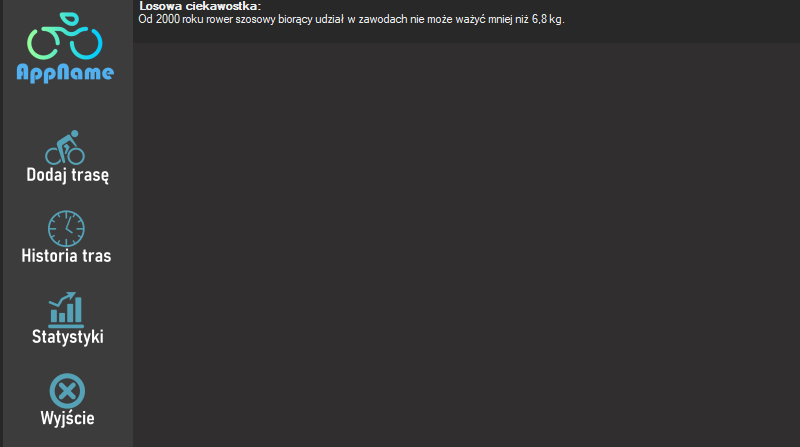
\includegraphics[width=15cm]{rys/main_screen.png}
		\caption{Propozycja ekranu głównego}
		\label{rys:Propozycja ekranu głównego}
	\end{center}
\end{figure}



   	\newpage
\section{Projektowanie}		%3
%Opis przygotowania narzędzi (git, visual studio). Wybór i opis bibliotek, klas. Szkic layoutów. Pseudo kody. Opisy wykorzystanych algorytmów (np. algorytm sortowania). Dokładniejsze określenie założeń i działania aplikacji, (np.: ten przycisk otworzy takie okno a w tym oknie wpisujemy takie dane).


\subsection
{Narzędzia}
\textit 
{
	Do wykonania aplikacji użyte zostaną następujące narzędzia: \\
	- Visual Studio 2019\\
	- Xamarin Forms v5.0.0.2125\\
	- GitHub\\
	- Nuget packages\\
	- Android Emulator(Pixel 2 Pie 9.0)
}

\textit
{\\
	%rysunek
	\begin{figure}[!htb]
		\begin{center}
			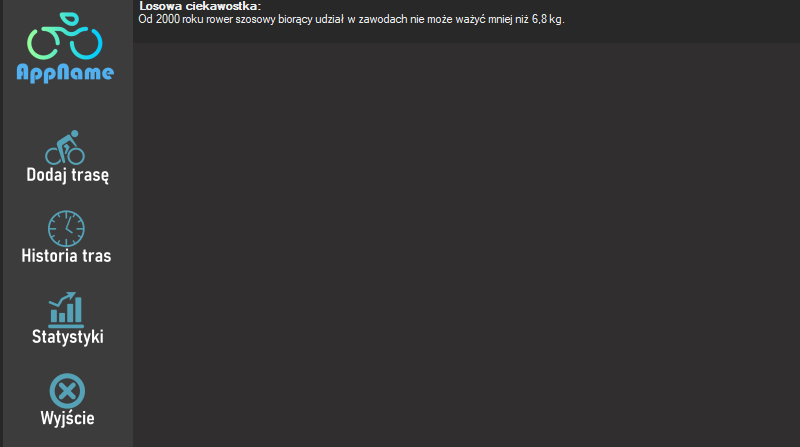
\includegraphics[width=15cm]{rys/main_screen.png}
			\caption{Szkic strony głównej aplikacji}
			\label{rys:Szkic strony głównej aplikacji}
		\end{center}
	\end{figure}
}

\newpage
\subsection
{Xamarin.Forms}
\textit
{
	Xamarin Forms to framework pozwalający pisać aplikacje na systemy takie jak m.in. Android oraz iOS. Łączy on głównie język C\# oraz XML.  Polega na budowaniu struktury komponentów 		składającej się z widoków, modeli widoków oraz zawartości (view(page), viewmodel, content) które służą do projektowania wyglądu oraz sposobu działania aplikacji.\\
	Struktura projektu (rozwiązania, wg. nazewnictwa wykorzytanego w projektowaniu środowiska Visual Studio) została zaprezentowana na rysunku 3.2.\\
	%rysunek
	\begin{figure}[!htb]
		\begin{center}
			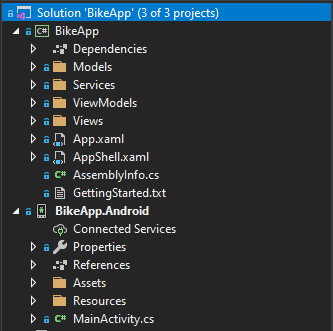
\includegraphics[width=10cm]{rys/xamarin_structure.png}
			\caption{Struktura projektu widoczna w programie Visual Studio}
			\label{rys:Struktura projektu widoczna w programie Visual Studio}
		\end{center}
	\end{figure}
}






   	\newpage
\section{Implementacja}		%4
%Wkleić szkielet kodu, wraz z komentarzami. Opisać zmienne, struktury do czego służą. Opisać procedury, metody co wykonują. Opisać nowe zdefiniowane klasy. Opisać dziedziczenie. Opisać nowo utworzone pliki za co odpowiadają.
\subsection{Pierwsze kroki}
\textit
{
	Po stworzeniu projektu poznawaliśmy strukturę oraz działanie aplikacji próbując modyfikować istniejące już klasy. Po zapoznaniu się z podstawami realizowaliśmy dalsze tutoriale aby 			swobodnie pracować w środowisku Xamarin'a.
}

\subsection{Modyfikacja menu}

\textit
{
	Pierwszym zadaniem było ustalenie szaty graficznej, widoku podstawowego z przyciskiem oraz menu. Aby to zrobić należało wykonać następujące czynności:\\\\
	-Dopisać odpowiednie właściwości do kodu XML typu background color, font-size, padding, textcolor itp. aby wystylizować układ widoku.\\\\
	Fragment modyfikacji:
	\begin{figure}[!htb]
		\begin{center}
			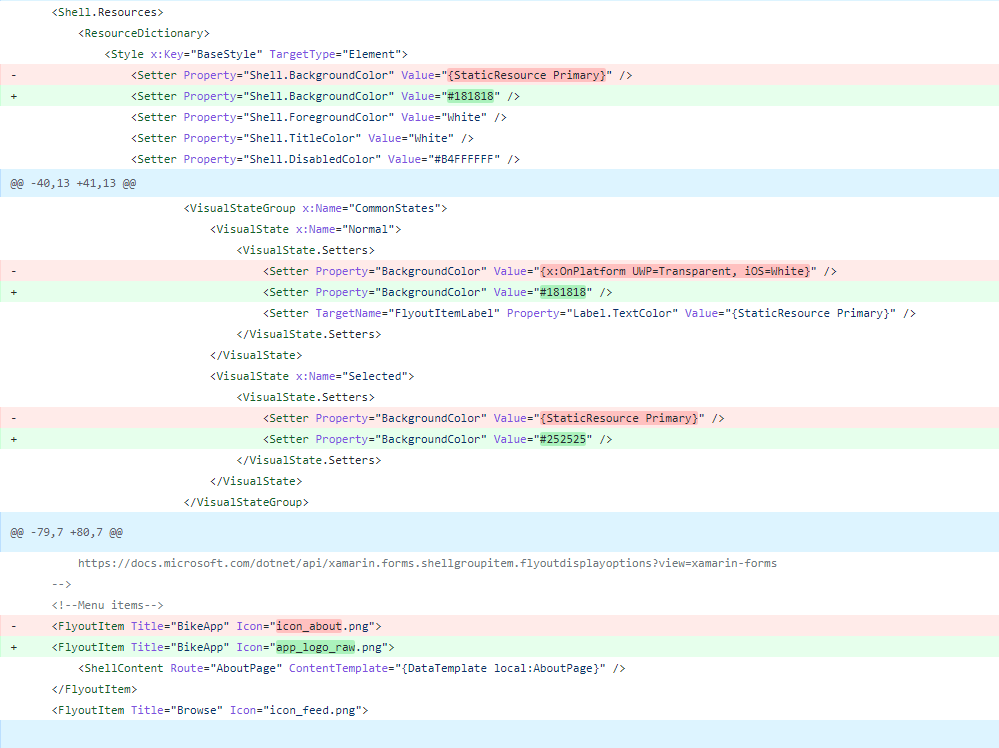
\includegraphics[width=15cm]{rys/gitchanges1.png}
			\caption{Zmiany styli}
			\label{rys:Zmiany styli}
		\end{center}
	\end{figure}
}

\newpage
\textit
{
	-Stworzyć widok główny na podstawie języka XML oraz metody w języku C\# informującej o kliknięciu w przycisk.\\\\
	Fragment modyfikacji:
	\begin{figure}[!htb]
		\begin{center}
			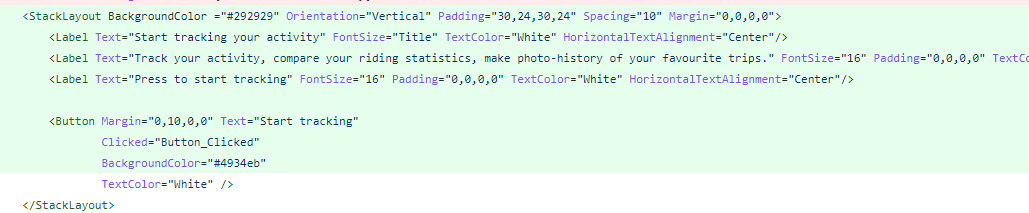
\includegraphics[width=15cm]{rys/gitchanges2.png}
			\caption{Implementacja widoku}
			\label{rys:Implementacja widoku}
		\end{center}
	\end{figure}
}

\textit
{
	-Pobrać i zainstalować paczkę 'acr' z nuget packages, zaimplementować opcję alertu, zaktualizować wersję xamarin.forms z 5.0.0.2012 do 5.0.0.2125 z powodu konfliktu biblioteki 				emulującej android w języku java \\\\
	Zmiany widoczne w kodzie:
	\begin{figure}[!htb]
		\begin{center}
			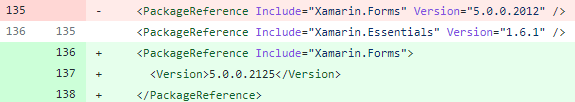
\includegraphics[width=15cm]{rys/gitchanges3.png}
			\caption{Modyfikacja nuget packages}
			\label{rys:Modyfikacja nuget packages}
		\end{center}
	\end{figure}
}




   	\newpage
\section{Testowanie}	%5
%Opisujemy testy, sprawdzamy czy nie generuje błędów.
\subsection{Menu} %5.1
Aby testowanie było bezproblemowe i kompleksowe należy przetestować każdą część aplikacji stopniowo zwiększając stopień skomplikowania. Pierwszym testem będzie działanie menu, składa się on z następującego scenariusza:\\\\
1)Otworzenie aplikacji\\
2)Sprawdzenie czy strona główna to widok zaimplementowany w klasie MainPage\\
3)Sprawdzenie czy każda opcja w menu pokrywa się z zaimplementowanym widokiem\\
4)Ustawienie aplikacji na działanie w tle, ponowne włączenie, i sprawdzenie czy otwiera się na ostatniej przeglądanej stronie\\
5)Przełączanie zakładek używając multitoucha\\\\
Wyniki: Aplikacja działa poprawnie, nie pojawia się żaden bug\\\\
\newpage
\subsection{Śledzenie trasy} %5.2
Scenariusz:\\
1)Otwarcie zakładki 'Start Tracking'\\
2)Wciśnięcie przycisku 'Start Tracking'\\
3)Sprawdzenie czy tekst na przycisku zmienił się na 'Stop Tracking'\\
4)Wciśnięcie przycisku 'Stop tracking' przed upływem 10 sekund od wciśnięcia 'Start Tracking'\\
5)Sprawdzenie czy przycisk spowrotem zmienił się na 'Start Tracking' oraz czy aplikacja nie zaproponowała zapisania trasy\\
6)Ponowne wciśnięcie przycisku 'Start Tracking' i odczekanie 10 sekund\\
7)Wciśnięcie przycisku 'Stop Tracking'\\
8)Sprawdzenie czy aplikacja zaproponowała zapisanie trasy\\
9)Zapisanie trasy\\
10)Sprawdzenie czy w zakładce 'My routes' została dodana trasa\\
11)Sprawdzenie czy trasa posiada poprawne wartości GPS z pozycji kodu\\\\
Wyniki: Wystąpił bug. Śledzenie trasy działa, ale pokazuje na mapie jedynie linię prostą z początku i końca śledzenia.\\\\
\newpage
\subsection{Wyświetlanie tras} %5.3
Scenariusz:\\
1)Otwarcie zakładki 'Your routes'\\
2)Sprawdzenie czy wcześniej dodane trasy poprawnie się wyświetlają\\
3)Sprawdzenie czy po kliknięciu na trasę wyświetlają się jej szczegóły oraz opcja jej usunięcia\\
4)Kliknięcie 'Display on map' oraz sprawdzenie czy wyświetla się poprawna trasa\\
5)Kliknięcie 'Delete', przełączenie się spowrotem na zakładkę 'Your routes' i sprawdzenie czy trasa się usunęła\\\\
Wyniki: Wystąpił bug. Trasa się usuwa, ale lista aktualizuje się dopiero po wyjściu z zakładki 'Your routes' oraz ponownym wejściu.
\subsection{Mapa} %5.4
Scenariusz:\\
1)Otwarcie zakładki 'Map'\\
2)Sprawdzenie mapa poprawnie się wyświetla\\
3)Kliknięcie opcji 'Update Location'\\
4)Sprawdzenie czy lokalizacja została uaktualniona, i czy aplikacja wycentrowała mapę na aktualnej lokalizacji\\
5)Sprawdzenie czy działa zoom za pomocą przycisków z ikonami + i -, oraz za pomocą gestu\\
6)Sprawdzenie czy działa uaktualnianie lokalizacji za pomocą ikony w prawym górnym rogu \\\\
Wyniki: Aplikacja działa poprawnie, nie pojawia się żaden bug\\\\
\newpage
\subsection{Pomiar rzeczywisty} %5.5
Scenariusz:\\
1)Otwarcie zakładki 'Live measurements'\\
2)Włączenie akcelerometra za pomocą slidera\\
3)Sprawdzenie czy po odpowiednim obrocie telefonu wartości się poprawnie wyświetlają. Wartość powinna wynosić zero jeśli telefon jest ustawiany prostopadle do siły grawitacji względem odczytywanej osi\\
4)Podrzucenie telefonu i sprawdzenie czy zmieniła się wartość maksymalnego zanotowanego przeciążenia G\\
5)Włączenie funkcji 'Shake Detection'\\
6)Kilkukrotne potrzęsienie telefonem i sprawdzenie czy pojawiło się okno z powiadomieniem 'Shake detected'
Wyniki: Aplikacja działa poprawnie, nie pojawia się żaden bug.

\subsection{Statystyki} %5.6
Scenariusz:\\
1)Dodanie za pomocą kodu tras z tak policzonymi wartościami aby dało się porównać ich statystyki liczone za pomocą aplikacji z wynikiem rzeczywistym\\
2)Otwarcie zakładki 'Statistics'\\
3)Sprawdzenie czy wszystkie pola tekstowe wyświetlają poprawne wartości(maksymalnie 2 miejsca po przecinku, poprawny format czasowy)\\
4)Porównanie wyników pokazywanych przez aplikacje z rzeczywistymi obliczeniami średnich na podstawie dodanych tras\\\\
Wyniki: Aplikacja działa poprawnie, nie pojawił się żaden bug\\\\

\newpage
\subsection{Ustawienia} %5.7
Scenariusz:\\
1)Uruchomienie aplikacji, sprawdzenie czy domyślnie jest włączony tryb ciemny\\
2)Otwarcie zakładki 'Settings'\\
3)Wyłączenie trybu ciemnego za pomocą slidera\\
4)Otwarcie po kolei każdej z zakładek i sprawdzenie czy tło jak i tekst wyświetlają się poprawnie w trybie jasnym\\
5)Otwarcie zakładki 'Settings'\\
6)Ponowne włączenie trybu ciemnego za pomocą slidera\\
7)Przejście po kolei każdej z zakładek i sprawdzenie czy tło jak i tekst wyświetlają się poprawnie w trybie ciemnym
Wyniki: Aplikacja działa poprawnie, nie pojawił się żaden bug\\\\


   	\newpage
\section{Podręcznik użytkownika}  %6
%Opis jak używać programu. Mogą być z zrzut ekranu razem z opisem. 

\subsection{Czym jest BikeApp?} %6.1

BikeApp jest aplikacją stworzoną dla rowerzystów wszelkiego rodzaju, od osób jeżdżących rekreacyjnie, przez turystów aż po zawodowych kolarzy (rysunek 6.1). Pozwala na zapisanie w pamięci telefonu różnych danych, które mogą być mu potrzebne, takich jak często odbywane trasy oraz dane pomiarowe. Oferuje przy tym prostą obsługę tych udogodnień oraz możliwość spersonalizowania ustawień.\\
\\
Niniejsza instrukcja zawiera informacje odnośnie korzystania z aplikacji, a w szczególności - komponentów, na które się ona składa.\\

\begin{figure}[!htb]
	\begin{center}
		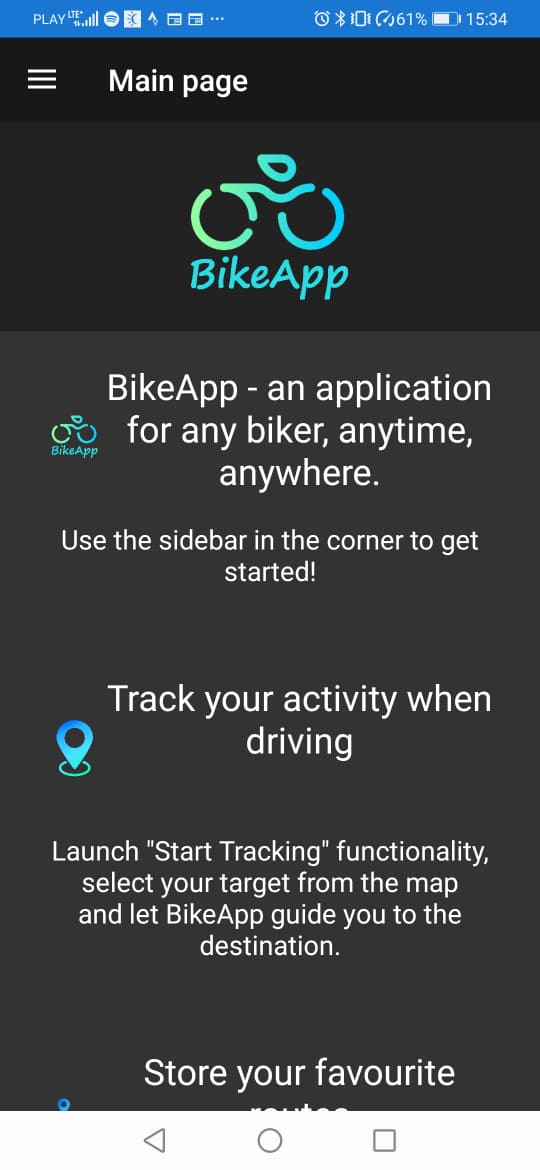
\includegraphics[width=6cm]{rys/instructions-mainpage.jpg}
		\caption{BikeApp - strona główna}
		\label{rys:BikeApp - strona główna}
	\end{center}
\end{figure}

\subsection{Dostęp do menu głównego oraz spis podstron} %6.2
Aplikacja BikeApp podzielona jest na podstrony, zaś dostęp do nich możliwy jest za pośrednictwem menu głównego.\\
\\
Menu główne jest otwierane przy użyciu znajdującej się w lewym górnym rogu ekranu ikony trzech poziomych linii. Jżeli zamiast niej widoczna jest strzałka, wówczas oznacza ona cofnięcie się do poprzedniej podstrony i należy ją wybierać i cofać się aż do pojawienia się ikony otwarcia menu głównego.\\
\\
Wybranie opcji na menu głównym (rysunek 6.2) spowoduje otwarcie właściwej podstrony poświęconej danej funkcji. Tematy obsługi poszczegónych podstron oraz opisu funkcji rozwinięto w dalszych podrozdziałach.

\begin{figure}[!htb]
	\begin{center}
		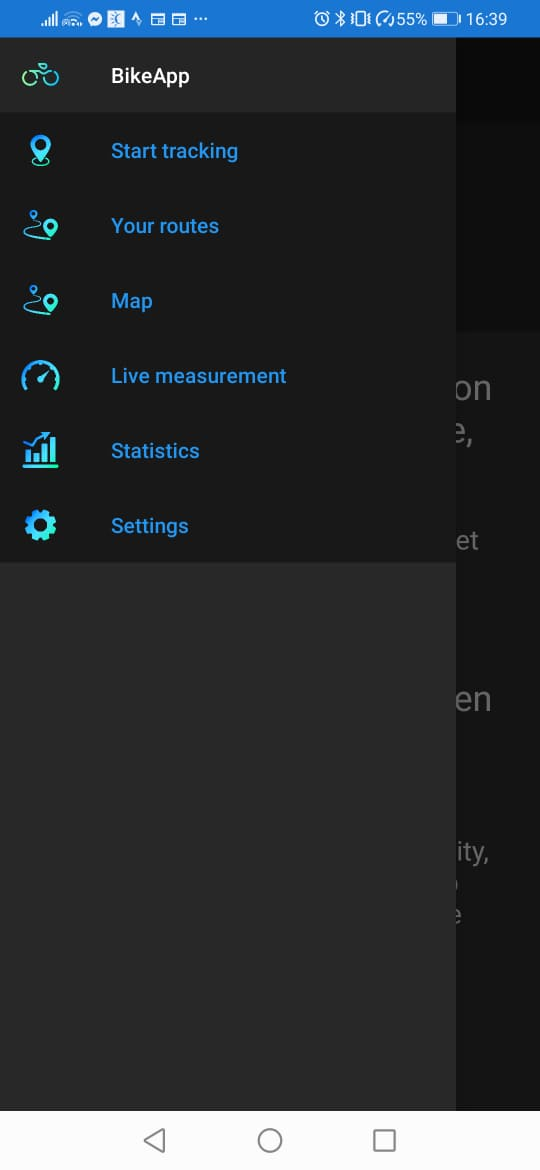
\includegraphics[width=6cm]{rys/instructions-menu.jpg}
		\caption{BikeApp - menu główne}
		\label{rys:BikeApp - menu główna}
	\end{center}
\end{figure}

\subsection{Mechanizm śledzenia trasy} %6.3
Tryb śledzenia trasy pozwala na zapisanie ścieżki, którą użytkownik przebędzie w trakcie jego działania. Powstała w ten sposób trasa może następnie zostać wyświetlona na mapie bądź zapisana w pamięci telefonu w celu późniejszego przeglądania.\\
\\
Aby uruchomić podstronę śledzenia trasy, należy rozwinąć menu główne i wybrać opcję ``Start Tracking''.\\
\\
Tryb śledzenia trasy jest uruchamiany poprzez wybranie przycisku ``Start tracking'' na podstronie (rysunek 6.3). Jego włączenie potwierdzi stosowny wyskakujący komunikat. Ponowne użycie tego samego przycisku zatrzymuje działanie trybu śledzenia trasy, a następnie wyświetla monit o nadanie trasie nazwy, po czym zostaje ona zapisana przez aplikację.\\
\\
W trakcie śledzenia trasy możliwe jest wykonywanie innych czynności na telefonie, w tym zamknięcie okna aplikacji i wyjście do ekranu głównego systemu telefonu.

\begin{figure}[!htb]
	\begin{center}
		
\includegraphics[width=6cm]{rys/instructions-tracking.jpg}
		\caption{BikeApp - podstrona śledzenia trasy}
		\label{rys:BikeApp - podstrona śledzenia trasy}
	\end{center}
\end{figure}

\subsection{Zarządzanie zapisanymi trasami} %6.4
Po zakończeniu śledzenia danej trasy, jest ona zapisywana pod nazwą wskazaną przez uzytkownika. Lista tras oraz parametry każdej z nich dostępne są z poziomu specjalnej podstrony.\\
\\
Aby obejrzeć zapisane trasy, należy rozwinąć menu główne i wybrać opcję ``Your Routes''.\\
\\
Każda pozycja na liście może zostać zaznaczona, co przeniesie użytkownika do ekranu z informacjami na temat wybranej trasy (rysunek 6.4). Aby powrócić do ekranu ze spisem zapisanych tras, należy uzyć strzałki znajdującej się w lewym górnym rogu. Działanie przycisku ``Display on Map'' opisano w podrozdziale ``Wyświetlanie trasy na mapie'' niniejszej instrukcji.

\begin{figure}[!htb]
	\begin{center}
		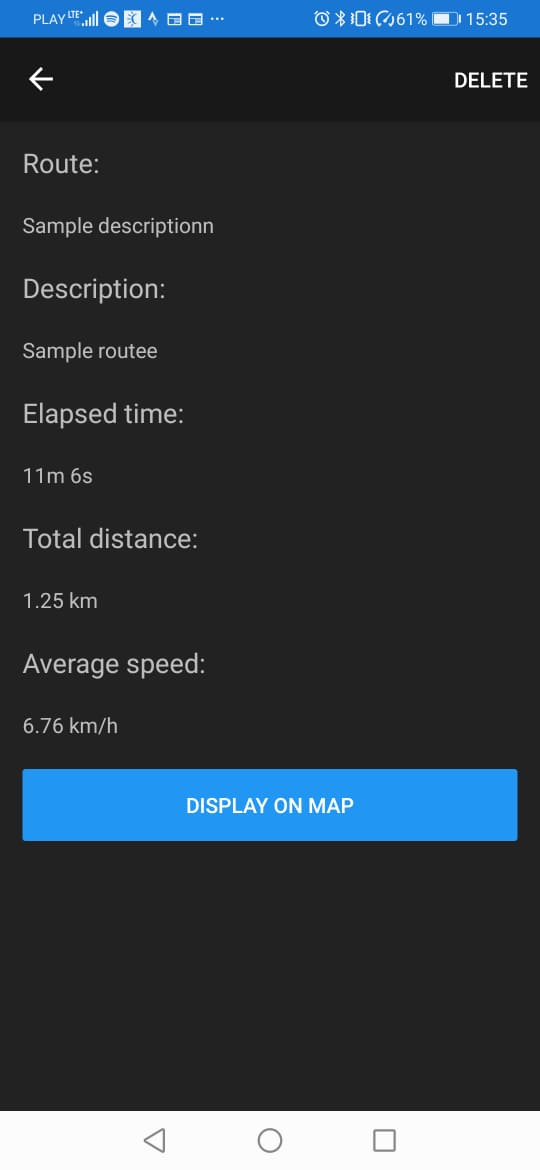
\includegraphics[width=6cm]{rys/instructions-route-details.jpg}
		\caption{BikeApp - szczegóły trasy}
		\label{rys:BikeApp - szczegóły trasy}
	\end{center}
\end{figure}

\subsection{Wyświetlanie trasy na mapie} %6.5
BikeApp zawiera podstronę z Mapą Google, dzięki której zapisane w pamięci telefonu trasy można obejrzeć w trybie graficznym. Będzie ona widoczna jako seria punktów połączonych prostymi liniami.\\
\\
Istnieją dwa sposoby na otwarcie Mapy Google wewnątrz aplikacji. Pierwszym jest wybranie opcji ``Map'' z menu głównego, drugim zaś - uruchomienie podstrony z listą tras, wybranie trasy oraz użycie przycisku ``Display on Map''. W przypadku sukcesu, widok będzie podobny, jak na rysunku 6.5.\\
\\
Przesuwanie oraz regulacja przybliżenia widoku na mapę odbywają się w sposób standardowy dla Map Google uruchamianych na urządzeniach mobilnych. Aplikacja nakłada również na mapę linie reprezentujące wybraną trasę.

\begin{figure}[!htb]
	\begin{center}
		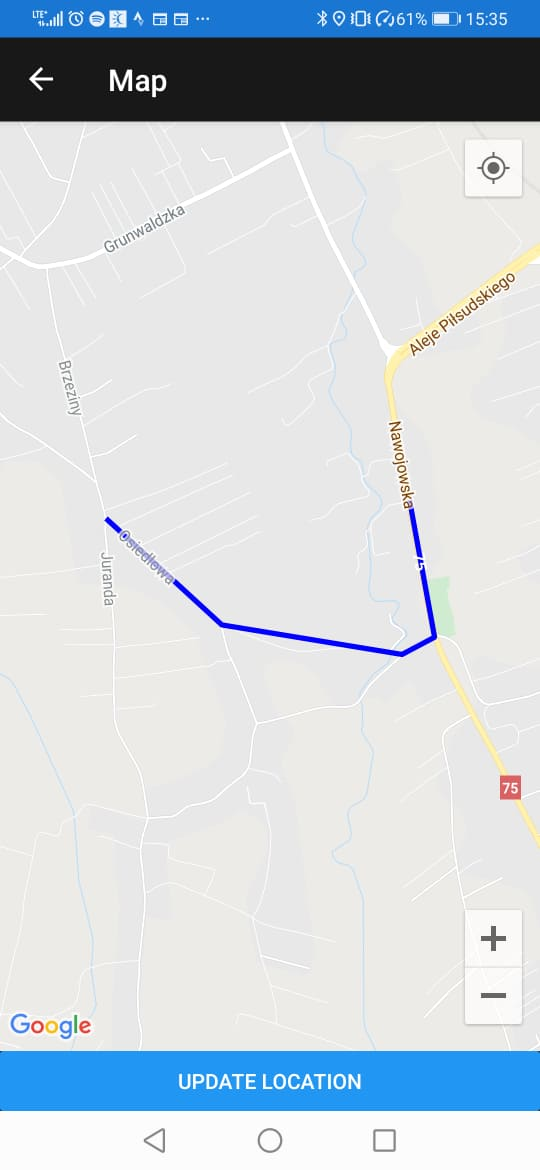
\includegraphics[width=6cm]{rys/instructions-map.jpg}
		\caption{BikeApp - Mapa Google}
		\label{rys:BikeApp - Mapa Google}
	\end{center}
\end{figure}

\subsection{Przeglądanie danych pomiarowych} %6.6
Aplikacja BikeApp może dokonywać pomiarów w trakcie jazdy. Mierzone są takie parametry jak kąty nachylenia urządzenia, przeciążenia oraz wystąpienia skoków przeciążeń, wynikających przykładowo z natrafienia na przeszkodę. Dane te mogą być wyświetlane na bieżąco bądź zbierane i przechowywane jako statystyki użytkownika.

\subsubsection{Dane chwilowe} %6.6.1
Aby uzyskać dostęp do danych wyświetlanych w momencie pobrania, należy z poziomu menu głównego wybrać pozycję ``Live measurement''. Użytkownikowi ukaże się podstrona wyglądająca tak, jak na rysunku 6.6.\\
\\
Pomiary danych są domyślnie zatrzymane po uruchomieniu aplikacji. Można je rozpocząć, korzystając z przełącznika odpowiadającego pozycji ``Accelerometer''. Poniżej przełączników będą widoczne zmierzone przez aplikację wartości.\\
\\
Drugi przełącznik, opisany nazwą ``Shake detection'', obsługuje wykrywanie skoków przeciążenia. Gdy jest ono aktywne, każdy moment, w którym pomiar przeciążenia wykaże odpowiednio wysoką wartość, będzie odnotowywany poprzez wyskakujące okienko. Wykrywania skoków przeciążenia nie można uruchomić, jeśli wyłączone jest także pobieranie danych chwilowych.

\begin{figure}[!htb]
	\begin{center}
		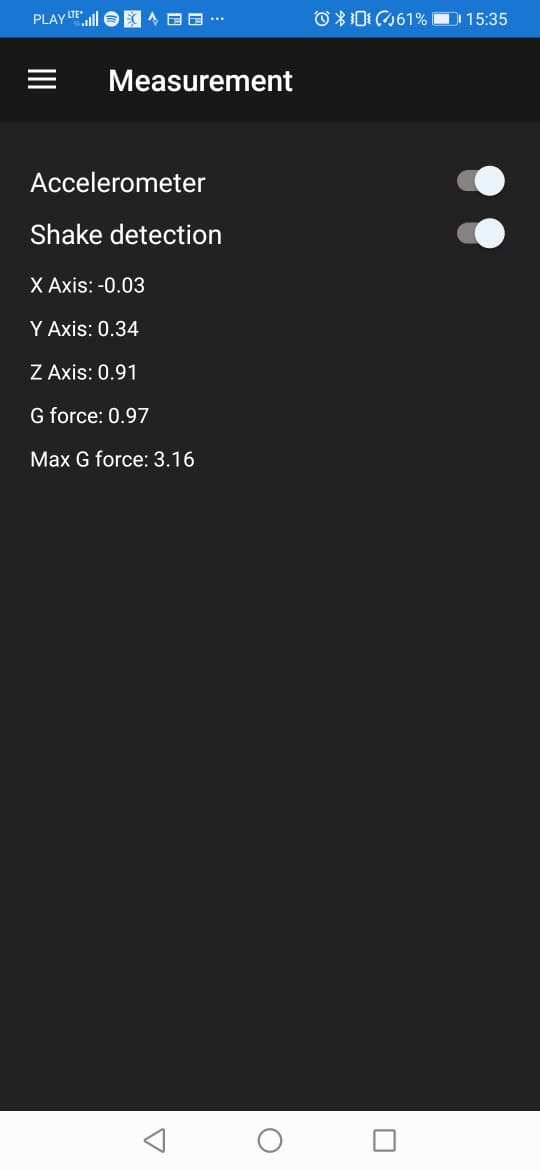
\includegraphics[width=6cm]{rys/instructions-measurement.jpg}
		\caption{BikeApp - Pomiary chwilowe}
		\label{rys:BikeApp - Pomiary chwilowe}
	\end{center}
\end{figure}

\subsubsection{Dane gromadzone w czasie (statystyki)} %6.6.1
Aby zobaczyć dane zbierane w dłuższym przedziale czasu, należy otworzyć menu główne i wybrać opcję ``Statistics''.\\
\\
Podstrona statystyk (rysunek 6.7) przedstawia różne rodzaje danych zgromadzonych przez aplikację w czasie, gdy tryb śledzenia trasy był aktywny. Obejmuje zarówno informacje o wartościach minimalnych i maksymalnych, jak również średnich.

\begin{figure}[!htb]
	\begin{center}
		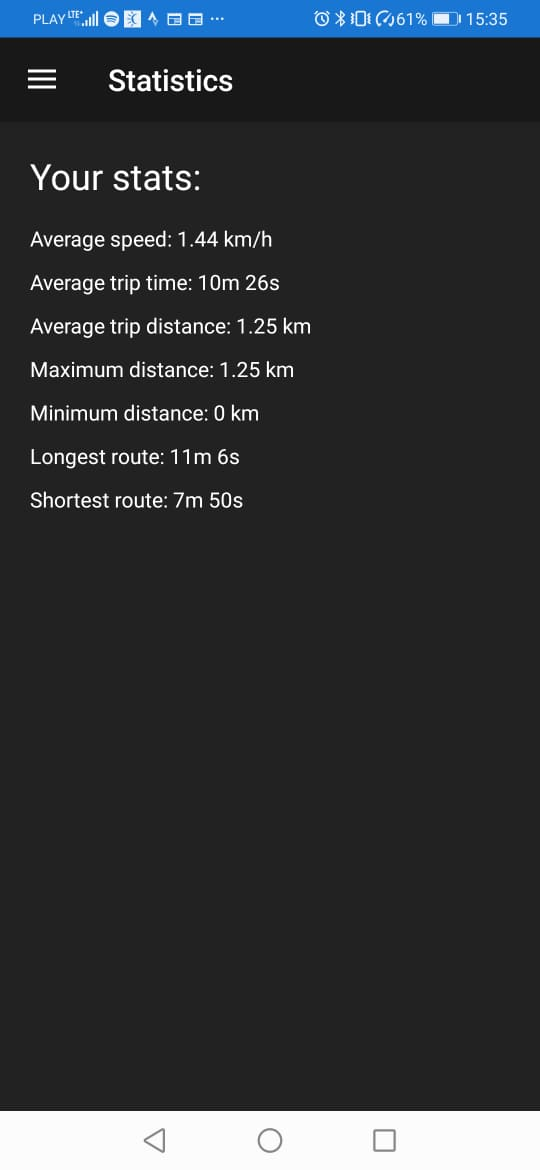
\includegraphics[width=6cm]{rys/instructions-stats.jpg}
		\caption{BikeApp - Podstrona statystyk}
		\label{rys:BikeApp - Podstrona statystyk}
	\end{center}
\end{figure}

\subsection{Dostosowanie ustawień} %6.7
Ustawienia aplikacji dostępne są za pośrednictwem menu głównego. Po jego otwarciu należy wybrać pozycję ``Settings''.\\
\\
Poszczególne opcje dostępne są w postaci przełączników, które można aktywować lub deaktywować poprzez ich użycie. Każda zmiana ustawień zatwierdzana jest natychmiast po jej wystąpieniu.

\newpage
\subsection{Częste problemy i błędy} %6.8
Większość problemów składa się z niekompatybilności wersji oraz dziwnego zachowania języka XAML względem języka C\#\\\\
Podstawowym problemem jest zachowanie się kolekcji w grid'zie znajdującym się z pliku XAML. Aby odświeżyć taką strukturę należy stworzyć zdarzenie w EventHandlerze, przypisać je do pola typu Command, wyczyścić stos zakładek, zaktualizować listę, wejść ponownie na zakładkę z gridem oraz połączyć to z wywołaniem XAML które koniecznie musi się wykonać zanim wczyta się viewmodel. Sposób ten wywołał tyle kłopotów i bugów, że zdecydowaśmy po prostu przeładowywać zakładkę ręcznie po usunięciu elementu z listy.\\\\\\

Kolejnym problemem jest nie do końca poprawne działanie serializacji na telefonie typu android. Mimo że typy proste są bez problemu zapisywane i odczytywane, to typy złożone wczytywane są z wartościami defaultowymi. Prowadzi to do konieczności konwersji do JSON'a, zapisywania struktury w postaci stringa, i ponownego przekonwertowywania po odczytaniu danych. Niestety rozwiązanie to generuje wiele bugów, więc spowodowało trudności w testowaniu aplikacji.\\\\

Problematyczne okazało się również konfigurowanie mapy, która wymagała klucza API od Google. Należało go skonfigurować zgodnie z używaną nazwą paczki i wieloma skomplikowanymi ustawieniami. Mimo poprawnych ustawień mapa nie działa na starszych urządzeniach(np. android 9.0)\\\\

Odświeżanie lokalizacji w trakcie śledzenia również sprawiło wiele problemów. Przy działaniu na jednym wątku aplikacja się zawieszała, generowała różne wyjątki lub zapisywała bezsensowne dane. Rozwiązanie przyszło dopiero po przeniesieniu śledzenia na drugi wątek oraz sygnału zakończenia śledzenia wysyłanego dopiero po zebraniu ostatniego sygnału.
 
   
       
%%%%%%%%%%%%%%%%%%% koniec treść główna dokumentu %%%%%%%%%%%%%%%%%%%%%
		\newpage
    \addcontentsline{toc}{section}{Literatura}  
	\printbibliography


    \newpage

    \hypersetup{linkcolor=black}
    \renewcommand{\cftparskip}{3pt}
    \clearpage
    \renewcommand{\cftloftitlefont}{\Large\bfseries\sffamily}
    \listoffigures
    \addcontentsline{toc}{section}{Spis rysunków}
	\thispagestyle{fancy}
    \newpage
    \renewcommand{\cftlottitlefont}{\Large\bfseries\sffamily}
    \def\listtablename{Spis tabel}%
    \addcontentsline{toc}{section}{Spis tabel}\listoftables 
	\thispagestyle{fancy}
	


    %lista rzeczy do zrobienia: wypisuje na koñcu dokumentu, patrz: pakiet todo.sty
    \todos
    %koniec listy rzeczy do zrobienia
\end{document}
